\begin{center}
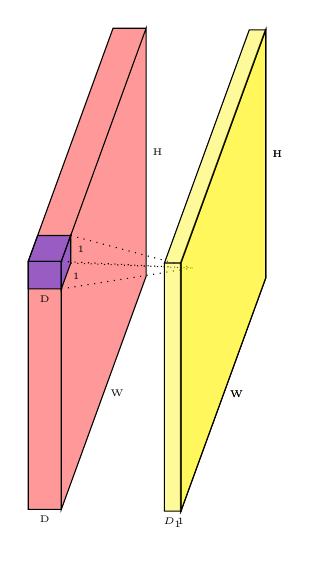
\begin{tikzpicture}[scale=0.7,transform shape]

\pgfsetxvec{\pgfpoint{1cm}{0cm}}
\pgfsetyvec{\pgfpoint{0cm}{1cm}}
\pgfsetzvec{\pgfpoint{-.342cm}{-.94cm}}

\def\cuboid#1#2#3#4#5{
\begin{scope}
\edef\mycolor{#2}
\edef\depth{#3}
\edef\height{#4}
\edef\width{#5}
\draw[black,fill=\mycolor, fill opacity=0.4, text opacity=1] #1 -- ++(-\depth,0,0) -- ++(0,-\height,0) -- ++(\depth,0,0) -- cycle #1 -- ++(0,0,-\width) -- ++(0,-\height,0) -- ++(0,0,\width) -- cycle  #1 -- ++(-\depth,0,0) -- ++(0,0,-\width) -- ++(\depth,0,0) -- cycle;
\end{scope}
}

\def\cuboidlabel#1#2#3#4#5#6#7#8{
\begin{scope}
\edef\mycolor{#2}
\edef\depth{#3}
\edef\height{#4}
\edef\width{#5}
\edef\depthlabel{#6}
\edef\heightlabel{#7}
\edef\widthlabel{#8}
\draw[draw=black,fill=\mycolor, fill opacity=0.4, text opacity=1] #1 -- ++(-\depth,0,0) -- ++(0,-\height,0) -- ++(\depth,0,0) node[pos=0.5,below] {\tiny \depthlabel} -- cycle #1 -- ++(0,0,-\width) -- ++(0,-\height,0) node[pos=0.5,right] {\tiny \heightlabel} -- ++(0,0,\width)  node[pos=0.5,below,right] {\tiny \widthlabel} -- cycle  #1 -- ++(-\depth,0,0) -- ++(0,0,-\width) -- ++(\depth,0,0) -- cycle;
\end{scope}
}

\def\kernel#1#2#3#4#5#6{
\begin{scope}
\edef\mycolor{#2}
\edef\depth{#3}
\edef\height{#4}
\edef\width{#5}
\draw[black,fill=\mycolor, fill opacity=0.4, text opacity=1] #1 -- ++(-\depth,0,0) -- ++(0,-\height,0) -- ++(\depth,0,0) -- cycle #1 -- ++(0,0,-\width) -- ++(0,-\height,0) -- ++(0,0,\width) -- cycle  #1 -- ++(-\depth,0,0) -- ++(0,0,-\width) -- ++(\depth,0,0) -- cycle;

\draw[dotted] #1 -- #6 #1++(0,0,-\width) -- #6 #1++(0,-\height,0) -- #6 #1++(0,-\height,-\width) -- #6;

\end{scope}
}

\def\kernellabel#1#2#3#4#5#6#7#8#9{
%#6 is target pixel
\begin{scope}
\edef\mycolor{#2}
\edef\depth{#3}
\edef\height{#4}
\edef\width{#5}
\edef\depthlabel{#7}
\edef\heightlabel{#8}
\edef\widthlabel{#9}
\draw[draw=black,fill=\mycolor, fill opacity=0.4, text opacity=1] #1 -- ++(-\depth,0,0) -- ++(0,-\height,0) -- ++(\depth,0,0) node[pos=0.5,below] {\tiny \depthlabel} -- cycle #1 -- ++(0,0,-\width) -- ++(0,-\height,0) node[pos=0.5,right] {\tiny \heightlabel} -- ++(0,0,\width)  node[pos=0.5,below,right] {\tiny \widthlabel} -- cycle  #1 -- ++(-\depth,0,0) -- ++(0,0,-\width) -- ++(\depth,0,0) -- cycle;

\draw[dotted] #1 -- #6 #1++(0,0,-\width) -- #6 #1++(0,-\height,0) -- #6 #1++(0,-\height,-\width) -- #6;

\end{scope}
}

%alexnet
\onslide<2->{
\cuboidlabel{(2,-0.5,-0.5)}{red}{0.6}{4.5}{4.5}{D}{H}{W}
}
\onslide<3->{
\kernellabel{(2,-0.5,-0.5)}{blue}{0.6}{0.5}{0.5}{(3.7,-2.5,-2.5)}{D}{1}{1}
}
\onslide<3>{
\cuboidlabel{(4,-1,-1)}{yellow}{0.01}{4.5}{4.5}{1}{H}{W}
}

%\onslide<6->{
%\kernellabel{(2,-1.5,-1.5)}{blue}{0.3}{0.5}{0.5}{(3.7,-2.5,-2.5)}{$D_1$}{1}{1}
%}
\onslide<4->{
\cuboidlabel{(4,-1,-1)}{yellow}{0.3}{4.5}{4.5}{$D_1$}{H}{W}
}
\end{tikzpicture}
\end{center}

